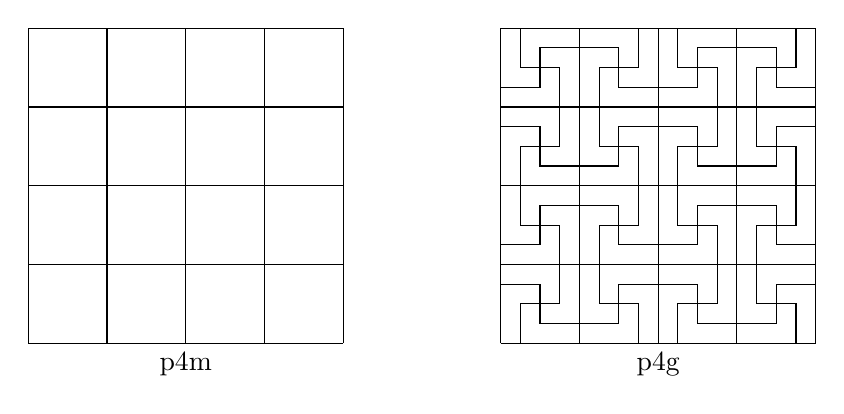
\begin{tikzpicture}[scale=1]

%draw left lattice

\coordinate (p4m-label) at (-3,0);
\node [below] at (p4m-label) {p4m};

\draw[step=1] (-5,0) grid (-1,4);

% draw right lattice

\coordinate (p4g-label) at (3,0);
\node [below] at (p4g-label) {p4g};

\draw[step=1] (1,0) grid (5,4);
\draw (1.25,0) -- (1.25,0.5) -- (1.75,0.5) -- (1.75,1.5) -- (1.25,1.5) -- (1.25,2.5) -- (1.75,2.5) -- (1.75,3.5) -- (1.25,3.5) -- (1.25,4);
\draw  (2.75,0) -- (2.75,0.5) -- (2.25,0.5) -- (2.25,1.5) -- (2.75,1.5) -- (2.75,2.5) -- (2.25,2.5) -- (2.25,3.5) -- (2.75,3.5) -- (2.75,4);
\draw   (3.25,0) -- (3.25,0.5) -- (3.75,0.5) -- (3.75,1.5) -- (3.25,1.5) -- (3.25,2.5) -- (3.75,2.5) -- (3.75,3.5) -- (3.25,3.5) -- (3.25,4);
\draw   (4.75,0) -- (4.75,0.5) -- (4.25,0.5) -- (4.25,1.5) -- (4.75,1.5) -- (4.75,2.5) -- (4.25,2.5) -- (4.25,3.5) -- (4.75,3.5) -- (4.75,4);

\draw  (1,0.75) -- (1.5,0.75) -- (1.5,0.25) -- (2.5,0.25) -- (2.5,0.75) -- (3.5,0.75) -- (3.5,0.25) -- (4.5,0.25) -- (4.5,0.75) -- (5, 0.75);
\draw  (1,1.25) -- (1.5,1.25) -- (1.5,1.75) -- (2.5,1.75) -- (2.5,1.25) -- (3.5,1.25) -- (3.5,1.75) -- (4.5,1.75) -- (4.5,1.25) -- (5, 1.25);

\draw  (1,2.75) -- (1.5,2.75) -- (1.5,2.25) -- (2.5,2.25) -- (2.5,2.75) -- (3.5,2.75) -- (3.5,2.25) -- (4.5,2.25) -- (4.5,2.75) -- (5, 2.75);
\draw (1,3.25) -- (1.5,3.25) -- (1.5,3.75) -- (2.5,3.75) -- (2.5,3.25) -- (3.5,3.25) -- (3.5,3.75) -- (4.5,3.75) -- (4.5,3.25) -- (5, 3.25);

\end{tikzpicture}

